\documentclass[addpoints,11pt]{exam}

\usepackage{alltt}
\usepackage[margin=1in]{geometry}   % set up margins
\usepackage[T1]{fontenc}
\usepackage[usenames,dvipsnames]{xcolor}
\usepackage{enumerate}              % fancy enumerate
\usepackage{amsmath}                % used for \eqref{} in this document
\usepackage{amsthm}
\theoremstyle{definition}
\newtheorem{exmp}{Example}[section]
\usepackage{verbatim}               % useful for \begin{comment} and \end{comment}
\usepackage{eurosym}                % used for euro symbol
\usepackage{caption} 
\usepackage{graphicx}
\graphicspath{{Figures/}}
\usepackage{subcaption}
\usepackage{color}
\usepackage{float}
\usepackage{amssymb}
\usepackage{sgamevar}
\usepackage{sgame}
\usepackage[colorlinks=true]{hyperref}
\hypersetup{colorlinks=true, citecolor=ForestGreen, linkcolor=BlueViolet, urlcolor=Magenta}

%Solutions or nah (blank next two lines out for no solutions, unblank #3)
%\printanswers
%\newcommand{\dd}[1]{\par {\textbf{\textcolor{red}{#1}}}}
\newcommand{\dd}[1]{}  


\setlength\parindent{0pt}
\unframedsolutions
\SolutionEmphasis{\color{red}}
\CorrectChoiceEmphasis{\color{red}}
\renewcommand{\choicelabel}{(\alph{choice})}
\newcommand{\blank}[0]{\underline{\hspace{3cm}}}
\pointformat{\bfseries[\thepoints]}
\pointpoints{pt}{pts}
\pointsinrightmargin

\begin{document}
	
\title{\textbf{Final Exam} \\ \dd{Solutions\\} \vspace{2 mm} {\large ECON 101}}
\author{Summer I 2016}
\date{}
\maketitle

\makebox[\textwidth]{Name:\enspace\hrulefill}
\\

\makebox[\textwidth]{ONYEN:\enspace\hrulefill}
\\

\makebox[\textwidth]{PID:\enspace\hrulefill}
\\

\makebox[\textwidth]{Honor Code Signature:\enspace\hrulefill}
	
\begin{center}
	\fbox{\fbox{\parbox{5.5in}{\centering
			This exam consists of 50 multiple choice questions and 1 short answer question. Multiple choice questions should be bubbled in on a scantron. Extra paper for scratch work is attached. The total number of points available on this exam is \textbf{100}.}}}
\end{center}

\section*{Multiple Choice [1.5 pts each]}

Choose the option that best answers the question given.

\begin{questions}
	
\question Consider Table \ref{tab1}. 

\begin{table}[h!]
	\centering
	\caption{Production in Utopia}
	\label{tab1}
	\begin{tabular}{c|c|c|c|c|c}        
		
		$t$ & $k$ & $y$ & $i$ & $d$ & $\hat{y}$ \\
		\hline
		0 &  &  & $x$ & $y$ & ---\\
		1 &  & & &  & $-.45\%$ \\
		2 &  & & & & $z$\\
	\end{tabular}
\end{table}

Under the assumptions of the Solow Model, which of the following is true?

\begin{choices}
\choice $x>y$ and $z>-.45\%$
\CorrectChoice $x<y$ and $z>-.45\%$
\choice $x>y$ and $z<-.45\%$
\choice $x<y$ and $z<-.45\%$
\end{choices}

\begin{solution}
If output growth is negative in period 1, then it must be that $i<d$ in period 0. Output growth approaches zero as the country moves towards its steady state, so $z>-.45\%$.
\end{solution}

\newpage

\question Suppose the supply curve for coffee mugs shifts such that the market price of coffee mugs decreases. Which of the following statements \underline{must} be true?

\begin{enumerate}[i.]
	\item Producer surplus decreases due to the lower price.
	\item Consumer surplus increases as existing buyers in the market pay lower prices on the mugs they were already willing to buy.
	\item New buyers enter the market as a result of the price decrease and realize surplus.
\end{enumerate}

\begin{choices}
	\choice i, ii, and iii
	\choice i and iii
	\choice i and ii
	\CorrectChoice ii and iii
\end{choices}

\begin{solution}
If supply shifts such that the price of mugs decreases, then supply for mugs increased. The decrease in price will increase surplus to consumers already in the market and will also yield surplus to new consumers entering the market. The effect on producer surplus is ambiguous: The price of mugs is lower, but seller costs decreased and there are more transactions taking place so PS could increase.
\end{solution}

\question Refer to Figure \ref{fig1}. 

\begin{figure}[h!]
	\centering
	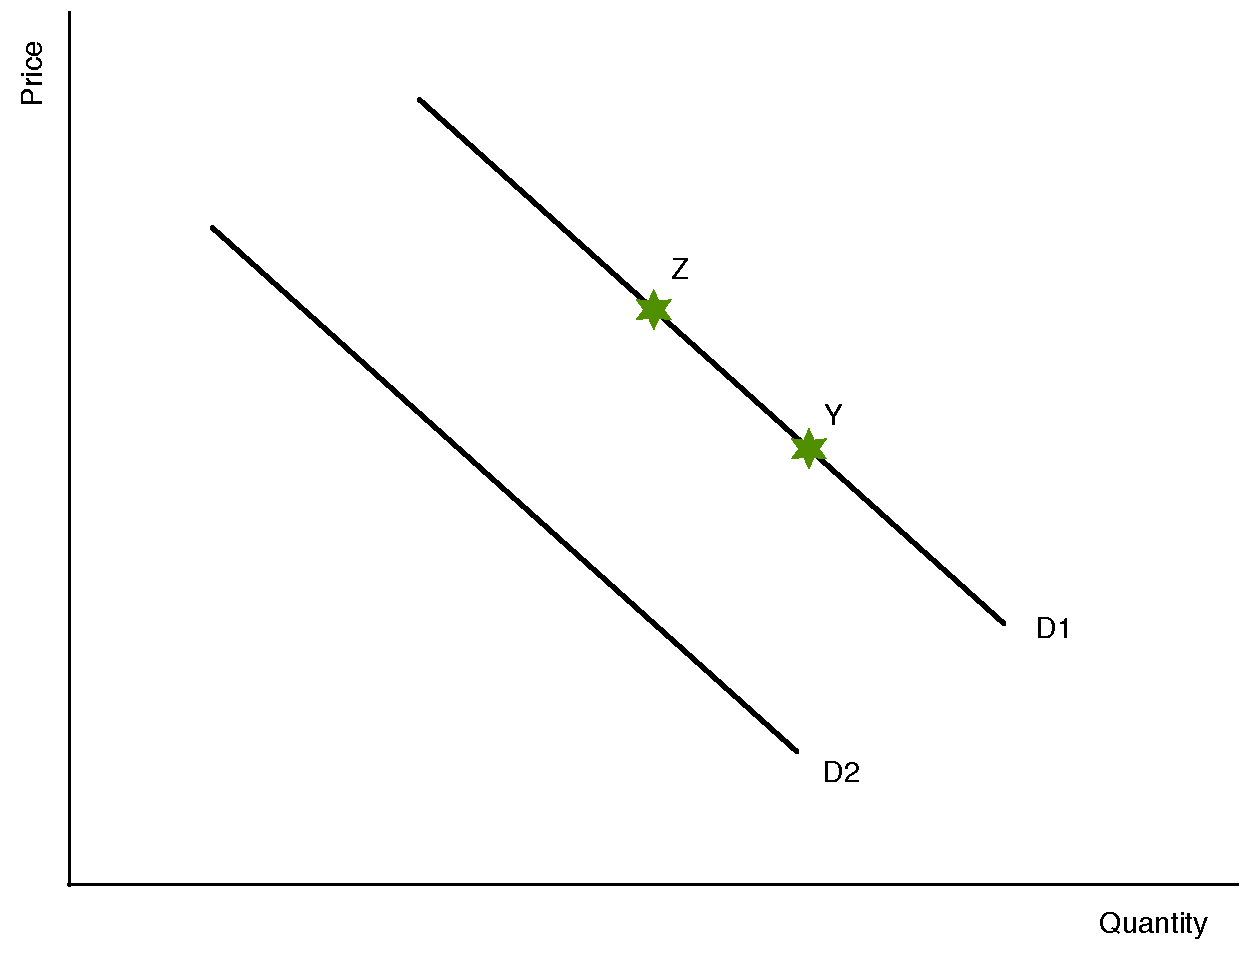
\includegraphics[scale=.35]{Exam1_MC2.pdf}
	\caption{Demand for Beer}
	\label{fig1}
\end{figure}

If the cross-price elasticity between beer and sausage is $-.45$, then an increase in the price of sausage will cause a move from

\begin{choices}
	\choice Z to Y
	\choice D2 to D1
	\CorrectChoice D1 to D2
	\choice Y to Z
\end{choices}

\begin{solution}
If the cross-price elasticity between beer and sausage is negative, then the goods are complements. An increase in the price of sausage will decrease demand for beer.
\end{solution}

\question Maple Leaf farm currently produces 1,000 bottles of syrup. The average total cost at this level of production is \$5.50, while the marginal cost of production is \$4.00. If the firm decides to increase production to 1,001 units, then the \blank at 1,001 units must be \blank. 

\begin{choices}
\choice ATC; greater than \$5.50
\choice MC; less than \$4.00
\choice MC; greater than \$5.50
\choice ATC; less than \$4.00
\CorrectChoice None of the above.
\end{choices}

\begin{solution}
If $ATC<MC$, then the average total cost must be decreasing. Thus, $ATC<\$5.50$.
\end{solution}

\question A country can produce either guns or butter and their production possibilities frontier is bowed out. If the country moves from a point where they are producing 25 guns and 30 pounds of butter to one where they are producing 35 guns and 30 pounds of butter, how many of the following statements could account for this?

\begin{enumerate}[i.]
	\item The country saw an influx of workers who specialize in making butter and moved from an efficient point on their former PPF to an efficient point on their new PPF.
	\item A technological breakthrough in gun production allowed the country to move from an efficient point on their former PPF to an efficient point on their new PPF. 
	\item The country moved from an efficient point on their PPF to another efficient point on the same PPF.
	\item The country moved from an inefficient point within their PPF to an efficient point on their PPF.
\end{enumerate}

\begin{choices}
	\choice 0
	\choice 1
	\choice 2
	\CorrectChoice 3
	\choice 4
\end{choices}

\begin{solution}
If the country is able to produce more guns without giving up any butter, then it cannot be moving along its PPF. i, ii, or iv could account for this, but not iii.
\end{solution}

\question You decide to put \$500 dollars into a savings account advertising 2\% annual interest. After a year, you withdraw your money and have to pay a tax of 20\% on your interest earnings. If inflation over the year was 1.75\%, then your after-tax nominal interest rate was \blank and your purchasing power \blank.

\begin{choices}
\choice .35\%; increased
\choice .6\%; decreased
\CorrectChoice 1.6\%; decreased
\choice .35\%; decreased
\choice 1.6\%; increased
\end{choices}

\begin{solution}
After-tax nominal interest rate = $2\%\times(1-.2)$ = 1.6\%. After-tax real return = 1.6\% - 1.75\% $<$ 0, so your purchasing power decreased.
\end{solution}

\question Bruce's Chum Shop calculates that changing the price of bait from \$2.10 to \$2.00 will increase their bait sales by 6\%. If they decide to go through with the price change, then their total revenue will

\begin{choices}
	\choice decrease because demand for bait is inelastic.
	\CorrectChoice increase because demand for bait is elastic.
	\choice increase because demand for bait is inelastic.
	\choice decrease because demand for bait is elastic.
\end{choices}

\begin{solution}
	$\%\Delta P = (2.10 - 2)/2.05 \times 100\% = 4.9\% < \%\Delta Q_d \Rightarrow$ Demand is elastic. Decreasing the price will increase total revenue.
\end{solution}

\newpage

\uplevel{Use Table \ref{tab2}, which shows how many hats or shirts Ben and Jerry can produce in a day, to answer questions \ref{q7} - \ref{q8}.}

\begin{table}[h!]
	\caption{Daily Production of Hats and Shirts}
	\centering
	\begin{tabular}{ c|c|c} 
		
		& Hats & Shirts \\
		\hline
		Ben & 15 & 10 \\
		Jerry & 12 & 9 \\
	\end{tabular}
	\label{tab2}
\end{table}

\begin{solution}
	Ben: 15 hats : 10 shirts $\Rightarrow$ 1 shirt : 1.5 hats. \\
	Jerry: 12 hats : 9 shirts $\Rightarrow$ 1 shirt : 1.33 hats. \\
	Jerry has CA in shirts, Ben has CA in hats. Jerry will export shirts and import hats. \\
	Terms of trade: 1 shirt : $X$ hats. \\
	Jerry only better off if $X>1.33$, Ben only better off if $X<1.5$. \\
	Acceptable terms of trade: $1.33 < X < 1.5$.
\end{solution}

\question \label{q7} Which of the following statements is TRUE?

\begin{choices}
\choice Ben has an absolute advantage in producing both shirts and hats, but Jerry has a comparative advantage in producing hats.
\choice Ben has a comparative advantage in producing shirts, while Jerry has a comparative advantage in producing hats.
\CorrectChoice Ben has an absolute advantage in producing shirts, but a comparative advantage in producing hats.
\choice None of the above are true.
\end{choices}

\question \label{q8} Suppose a terms of trade is given where 150 shirts will be exchanged for 270 hats. Is this an acceptable terms of trade for both parties?

\begin{choices}
	\CorrectChoice No. Ben would be worse off.
	\choice No. Both parties would be worse off.
	\choice No. Jerry would be worse off.
	\choice Yes. Both parties would be better off.
\end{choices}

\begin{solution}
TOT: 150 shirts : 270 hats $\Rightarrow$ 1 shirt : 1.8 hats. Jerry would be better off under these terms, but Ben would be worse off.
\end{solution}


\question Zuutopia experienced negative growth of real GDP per capita in the last year. Which of the following can explain this?

\begin{choices}
\choice The country's population shrunk over the last year while real GDP remained the same.
\choice The country's population grew over the last year while real GDP also increased but by a greater percentage.
\choice The country's population remained the same over the last year while real GDP increased.
\CorrectChoice The country's population grew over the last year while real GDP also increased but by a smaller percentage.
\end{choices}

\begin{solution}
$\hat{y} \approx \hat{Y} - \hat{N}$. If real GDP per capita fell over the last year, then $\hat{Y} < \hat{N}$. (d) is the only choice for which this holds true.
\end{solution}


\question Which of the following is an example of a negative real shock?

\begin{choices}
\choice Consumers become pessimistic about the economy and spend less.
\CorrectChoice A hurricane destroys numerous factories along the shoreline.
\choice The Federal Reserve is concerned about inflation and decreases the money supply.
\choice The government increases taxes on consumers.
\choice All of the above. 
\end{choices}

\newpage

\begin{solution}
See class notes.
\end{solution}

\question Refer to Figure \ref{fig2}.

\begin{figure}[h!]
	\centering
	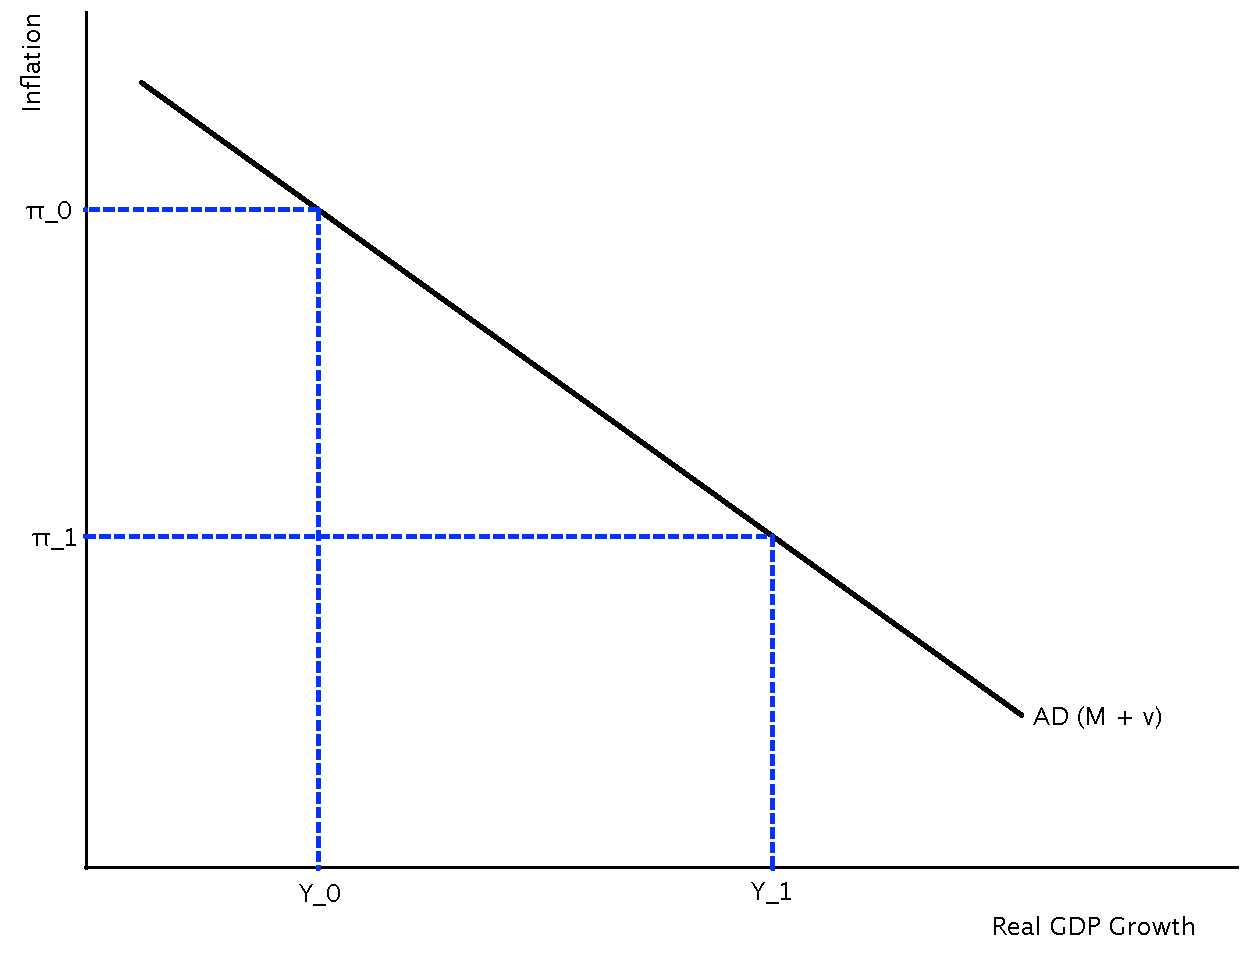
\includegraphics[scale=.40]{plot95.pdf}
	\caption{Aggregate Demand Curve}
	\label{fig2}
\end{figure}

Which of the following statements is correct?

\begin{choices}
	\choice $\pi_0 + \pi_1 = \vec{Y_0} + \vec{Y_1}$.
	\choice $\pi_0 + \vec{Y_1} = \pi_1 + \vec{Y_0}$.
	\choice $\pi_0 + \vec{Y_1} = \vec{M} + \vec{v}$.
	\choice $\pi_1 + \vec{Y_0} = \vec{M} + \vec{v}$.
	\CorrectChoice None of the above.
\end{choices}

\begin{solution}
	Along the given AD curve, spending growth = $\vec{M} + \vec{v} = \pi_0 + \vec{Y_0} = \pi_1 + \vec{Y_1}$.
\end{solution}

\question Jack loses his job working as a consultant and decides to take time off to explore Europe. Jill has been looking for work for some time, but gave up looking for a job 2 months ago. Given this, Jack's actions will \blank the employment rate while Jill's will \blank the unemployment rate.

\begin{choices}
\CorrectChoice increase; decrease
\choice increase; increase
\choice decrease; increase
\choice	decrease; decrease
\choice None of the above
\end{choices}

\begin{solution}
Jack goes from employed to out of the labor force: \#U remains the same, while \#LF falls $\Rightarrow$ unemployment rate = \#U/\#LF will increase. \\
Jill goes from unemployed to out of the labor force: \#U \& \#LF both decrease. Unemployment rate will increase since change in numerator will have a bigger effect.
\end{solution}

\question It takes Hannah 2 hours to bake a cake, while a batch of chocolate chip cookies takes 30 minutes to make. The opportunity cost to Hannah of making a batch of chocolate chips cookies is

\begin{choices}
\choice 1/15 cake. 
\choice 4 cakes.
\choice 15 cakes.
\CorrectChoice 1/4 cake.
\end{choices}

\begin{solution}
1 cake/120 minutes : 1 batch of cookies/30 minutes $\Rightarrow$ 1 batch of cookies : 30/120 cakes $\Rightarrow$ 1 batch of cookies : 1/4 cake.
\end{solution}

\question Suppose the Fed sets the minimum reserve ratio at 25\%. If banks choose to hold excess reserves and the Fed increases the money supply by \$5 million, then the maximum amount the money supply could potentially increase is

\begin{choices}
\choice exactly \$20 million.
\choice more than \$20 million.
\choice more than \$20 million but less than \$125 million.
\choice more than \$125 million.
\CorrectChoice None of the above.
\end{choices}

\begin{solution}
If banks hold excess reserves, then $rr>.25 \Rightarrow MM<5$, so the potential increase in the MS is less than \$20 million.
\end{solution}

\question The production function $F(K,L)$ has the property such that $F(3K,3L) = 3F(K,L)$. What is this property called?

\begin{choices}
\choice Increasing returns to scale.
\CorrectChoice Constant returns to scale.
\choice Diminishing marginal returns.
\choice Decreasing returns to scale.	
\end{choices}

\begin{solution}
See class notes.
\end{solution}

\question Cosmic is a firm in a perfectly competitive environment outlined in Figure \ref{fig3}.

	\begin{figure}[h!]
		\centering
		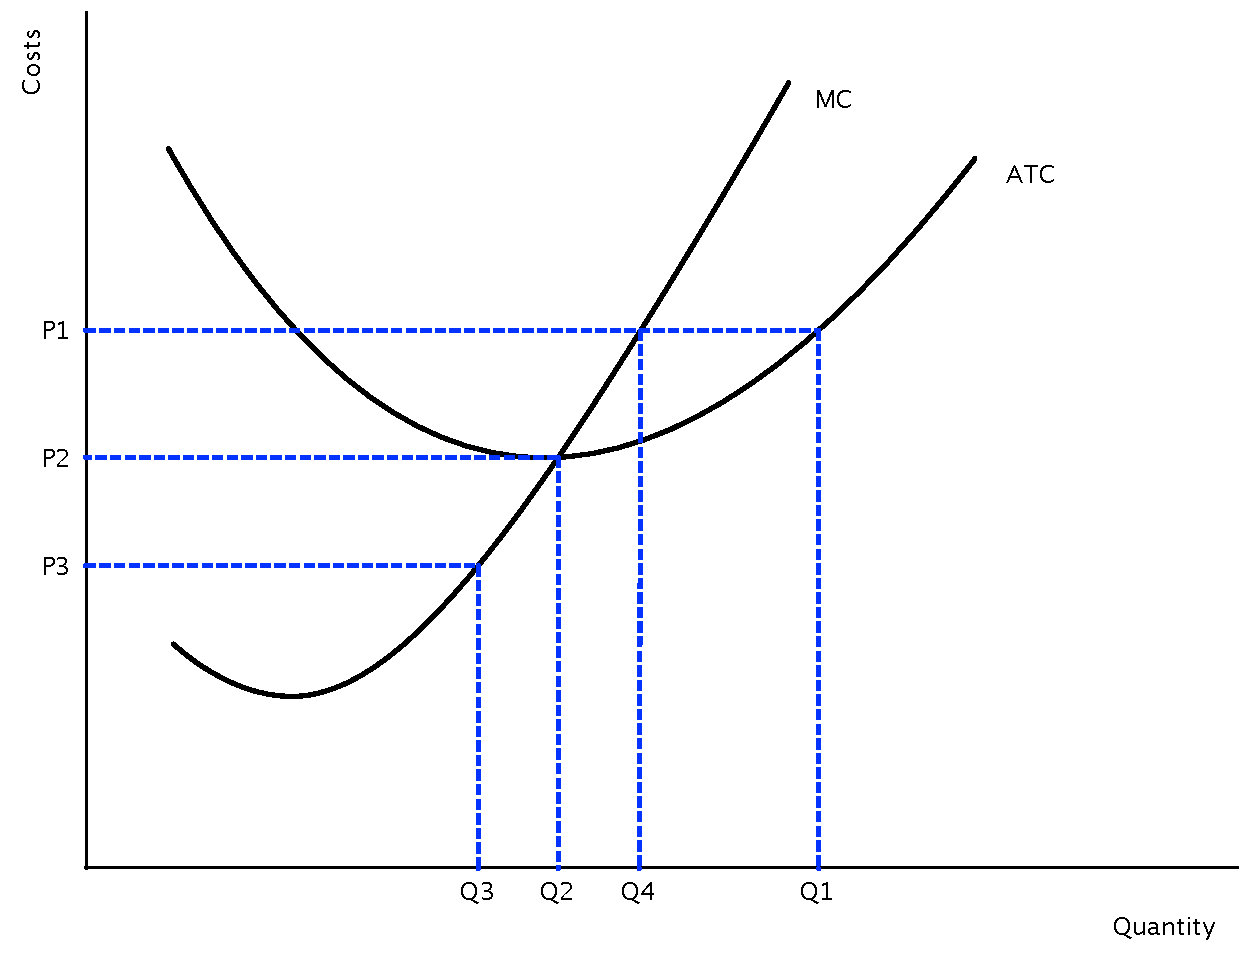
\includegraphics[scale=.40]{final_17.pdf}
		\caption{Environment Faced by Cosmic}
		\label{fig3}
	\end{figure}
	
If the price in the market is $P1$, then the firm will choose to produce \blank units of output. Additionally, the long-run price in the market will be \blank.
	
\begin{choices}
\choice $Q1$; $P2$
\choice $Q2$; $P3$
\choice $Q1$; $P1$
\CorrectChoice $Q4$; $P2$
\choice None of the above.
\end{choices}

\begin{solution}
Produce $Q$ where $P = MC$. Long-run price is at min $ATC$.
\end{solution}

\newpage

\question The equilibrium price for bobble head pumpkins is \$1.25. Suppose that the government imposes a price ceiling of \$1.00. Due to this price ceiling, producer surplus will \blank and total surplus will \blank.

\begin{choices}
\CorrectChoice decrease; decrease
\choice increase; decrease
\choice decrease; increase
\choice increase; increase
\choice remain unchanged; remain unchanged
\end{choices}

\begin{solution}
The price ceiling is below the market price, so it is binding. This will decrease both PS and TS in the market.
\end{solution}

\question Consider Table \ref{tab3}. 

	\begin{table}[h!]
		\caption{Market for Pencils}
		\centering
		\begin{tabular}{ c|c} 
			
			WTP & Seller Cost \\
			\hline
			\$6.25 & \$1.00  \\
			\$4.00 & \$3.00  \\
			\$3.50 & \$3.25  \\
			\$3.40 & \$3.40  \\
			\$3.00 & \$4.00  \\
		\end{tabular}
		\label{tab3}
	\end{table}
	
If the government imposes a per unit tax of \$1 on pencil sellers, then the quantity bought and sold will be \blank and \blank. 
	
\begin{choices}
\choice 2; sellers will bear more of the tax burden.
\choice 5; sellers will bear more of the tax burden.
\CorrectChoice 2; buyers will bear more of the tax burden.
\choice	2; buyers and sellers will split the tax burden evenly.
\choice 4; buyers will bear more of the tax burden.
\end{choices}
	
\begin{solution}
New quantity: 2 (tax wedge = \$1). Buyers now pay \$4, sellers receive \$3. Buyers bear \$.60 of the tax, sellers bear \$.40.
\end{solution}

\question A closed economy has private savings equal to \$500 billion and public savings of $-\$20$ billion. If consumption in the economy is \$400 billion and taxes equal \$50 billion, then government spending is \blank billion and total spending (i.e., GDP) in the economy is \blank billion.

\begin{choices}
\choice \$50; \$950
\choice \$70; \$900
\choice \$30; \$600
\CorrectChoice \$70; \$950
\end{choices}

\begin{solution}
Public savings: $T - G = 50B - G = -20B \Rightarrow G = 70B$. \\
Private savings: $Y - C - T = Y - 400B - 50B = 500B \Rightarrow Y = 950B$.
\end{solution}

\question If the government wishes to enact contractionary fiscal policy, it could

\begin{choices}
\choice increase both taxes and government spending. 
\choice reduce taxes or increase government spending.
\choice decrease both taxes and government spending.
\CorrectChoice increase taxes or reduce government spending.
\end{choices}

\begin{solution}
See class notes.
\end{solution}

\newpage

\question A firm operates in the market environment shown in Table \ref{tab4}. 

	\begin{table}[h!]
		\caption{Market for Jello}
		\label{tab4}
		\centering
		\begin{tabular}{ c|c|c} 
			
			$P$ & $Q_d$ & Total Cost \\
			\hline
			\$6.25 & 0 & \$2  \\
			\$4.00 & 2 & \$3 \\
			\$3.00 & 4 & \$6 \\
			\$2.50 & 6 & \$10\\
			\$1.00 & 8 & \$16  \\
		\end{tabular}
	\end{table}
	
The firm should produce \blank units of output and will make \blank in profit.
	
\begin{choices}
\CorrectChoice 4; \$6
\choice 6; \$5
\choice 4; \$12
\choice 6; \$15
\choice None of the above.
\end{choices}

\begin{solution}
Find where MR = MC. $Q^* = 4$, $\Pi = TR - TC = \$6$.
\end{solution}

\question Refer to Figure \ref{fig4}.

\begin{figure}[h!]
	\centering
	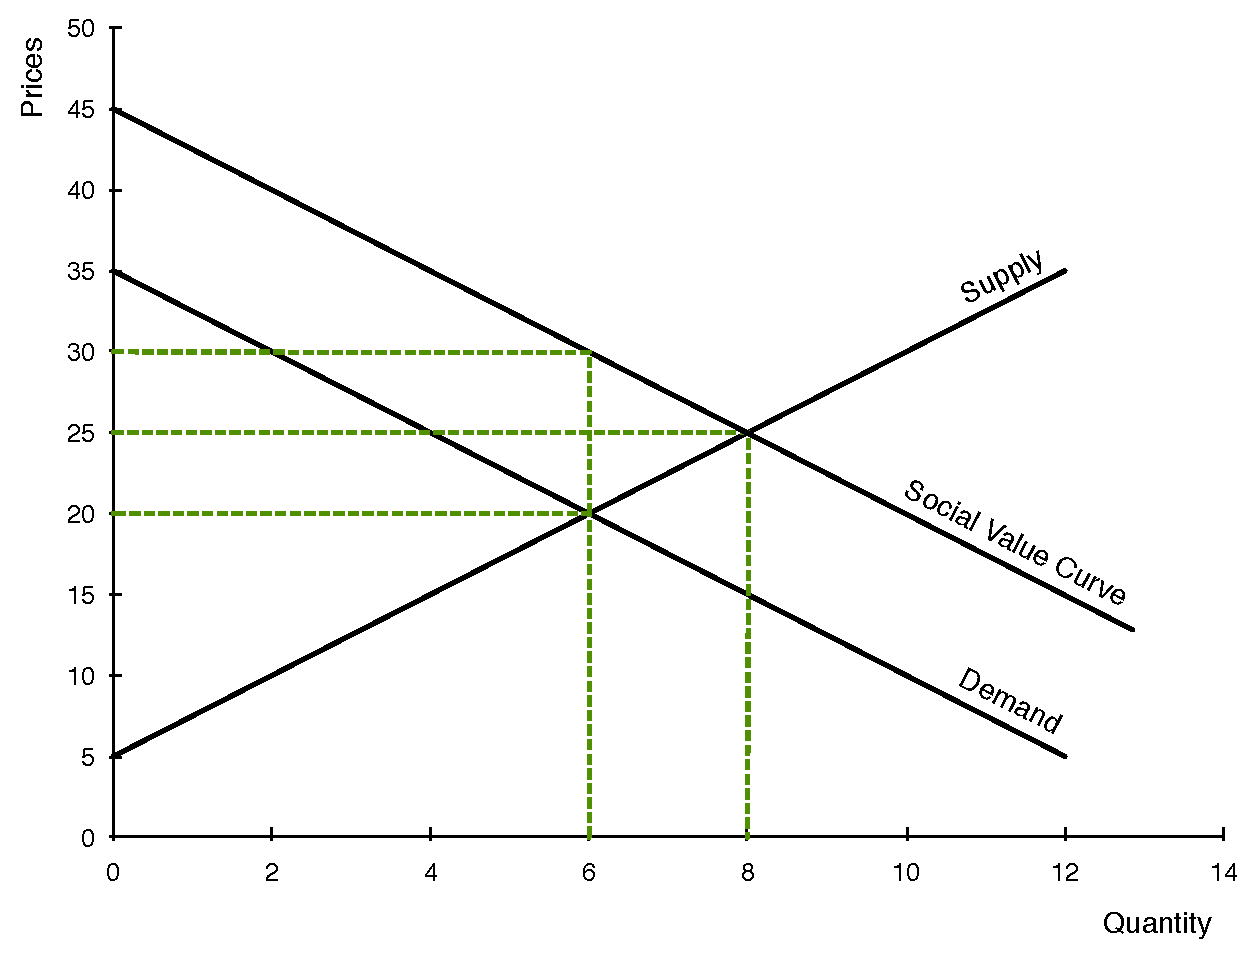
\includegraphics[scale=.40]{Exam_Review5.pdf}
	\caption{A Market Externality}
	\label{fig4}
\end{figure}

The socially efficient quantity is \blank, but in the absence of government intervention the market will have a deadweight loss of \blank.

\begin{choices}
\choice 6; \$10
\choice 8; \$20
\CorrectChoice 8; \$10
\choice 6; \$20
\end{choices}

\begin{solution}
Social efficient point where sv curve = supply curve. DWL = $(1/2)\times 2\times 10 = 10$.
\end{solution}

\newpage

\question How many of the following will lead to bias in the unemployment rate?

\begin{enumerate}[i.]
	\item Woody leaves his job at UNC and starts his own toy shop business.
	\item Morgan wishes to have a job, but stopped looking for work due to few call backs.
	\item Jonathan isn't actively looking for work, but claims to do so in order to receive unemployment benefits.
	\item Allen is fired from his job at McDonald's and immediately begins looking for work at other fast food joints.
\end{enumerate}

\begin{choices}
\choice 0
\choice 1
\CorrectChoice 2
\choice 3
\choice 4
\end{choices}

\begin{solution}
See class notes. ii and iii will lead to bias in the unemployment rate.
\end{solution}

\question You buy a bond today that promises to pay \$50 in one year, \$50 in two years, and \$1,050 in three years. If the market interest rate is 6\% and remains so for the next three years, which of the following represents the price of the bond if you decide to sell it in one year after receiving the first \$50 payment?

\begin{choices}
\choice $P = \frac{\$50}{(1.06)} + \frac{\$50}{(1.06)^2} + \frac{\$1,050}{(1.06)^3}$
\CorrectChoice $P = \frac{\$50}{(1.06)} + \frac{\$1,050}{(1.06)^2}$
\choice $P = \$50 + \frac{\$50}{(1.06)} + \frac{\$1,050}{(1.06)^2}$
\choice $P = \$50 + \frac{\$1,050}{(1.06)}$
\choice None of the above.
\end{choices}

\begin{solution}
See class notes. The price of a bond is the present value of its future payments.
\end{solution}

\question Which of the following is NOT a determinant of a country's long-run productivity?

\begin{choices} 
\choice Human capital
\choice Technological knowledge
\CorrectChoice Money supply
\choice Natural resources
\end{choices} 

\begin{solution}
See class notes.
\end{solution}

\question Suppose the government increases its purchases by 4\%. If the multiplier effect is greater than the crowding out effect, then

\begin{choices}
\choice the aggregate supply curve shifts to the right by more than 4\%.
\choice the aggregate supply curve shifts to the left by less than 4\%.
\CorrectChoice the aggregate demand curve shifts to the right by more than 4\%.
\choice the aggregate demand curve shifts to the left by more than 4\%. 
\end{choices}

\begin{solution}
An increase in govt. spending increases AD. If the multiplier effect is greater than the crowding out effect, AD will shift by more than the change in govt. spending.
\end{solution}

\newpage

\question Which of the following is true with regard to the pricing and production decisions of firms in monopolistically competitive markets? Monopolistically competitive firms produce

\begin{choices}
\choice at the efficient scale and charge a price equal to marginal cost.
\choice at the efficient scale and charge a price above marginal cost.
\choice with excess capacity and charge a price equal to marginal cost.
\CorrectChoice with excess capacity and charge a price above marginal cost.
\end{choices}

\begin{solution}
See class notes.
\end{solution}

\question How many of the following situations would unambiguously decrease the equilibrium price of milk today, which is a normal good?

\begin{enumerate}[i.]
	\item A technological advance allows milk farmers to produce milk at a lower cost.
	\item A prominent basketball player joins a new campaign that promotes the benefits of drinking milk.
	\item A famine wipes out half of milk producing cows.
	\item Both consumers and producers hear news that the price of milk will be lower next month.
\end{enumerate}

\begin{choices}
\choice 0
\choice 1
\CorrectChoice 2
\choice 3
\choice 4
\end{choices}

\begin{solution}
In order for the price of milk to fall, the supply of milk must increase, the demand for milk must decrease, or both must occur simultaneously. i and iv are the two options where this occurs.
\end{solution}

\question David is debating how many beers he should buy after grading his Econ 101 final exams. Table \ref{tab5} shows his willingness to pay for each additional beer as well as the total cost of each beer which includes the price of the beer along with the dollar cost of headache medicine, lost time, etc. each beer would have. 

	\begin{table}[h!]
		\caption{WTP and Costs of Beer}
		\label{tab5}
		\centering
		\begin{tabular}{ c|c|c} 
			
			Beer & WTP & Total Cost \\
			\hline
			1st & \$6.00 & \$4.50  \\
			2nd & \$6.00 & \$9.50 \\
			3rd & \$5.50 & \$15.00 \\
			4th & \$5.25 & \$21.00\\
			5th & \$5.00 & \$27.50  \\
			6th & \$4.50 & \$34.50 \\
		\end{tabular}
	\end{table}
	
Given this information, how many beers should he buy?
	
\begin{choices}
\choice No more than 1 beer.
\choice Exactly 2 beers.
\CorrectChoice Exactly 3 beers.
\choice Exactly 4 beers.
\choice At least 5 beers.
\end{choices}

\begin{solution}
WTP = MB of each beer. Use TC to find MC. Optimal amount is where $MB = MC =\$5.50$ at $Q=3$.
\end{solution} 

\newpage

\question Which of the following statements regarding elasticity is FALSE?

\begin{choices}
\CorrectChoice If the income elasticity of demand for some good is $-.75$, an increase in incomes will increase the quantity demanded for that good.
\choice A relatively elastic supply curve will have a smaller slope than a relatively inelastic supply curve.
\choice A perfectly inelastic demand curve implies that the price elasticity of the good is zero.
\choice Due to the Law of Supply, the price elasticity of supply is always positive.
\choice If the cross-price elasticity between two goods is positive, then an increase in the price of one will lead the an increase in quantity demanded for the other.
\end{choices} 

\begin{solution}
See class notes.
\end{solution}

\question Refer to Figure \ref{fig5}.

\begin{figure}[h!]
	\centering
	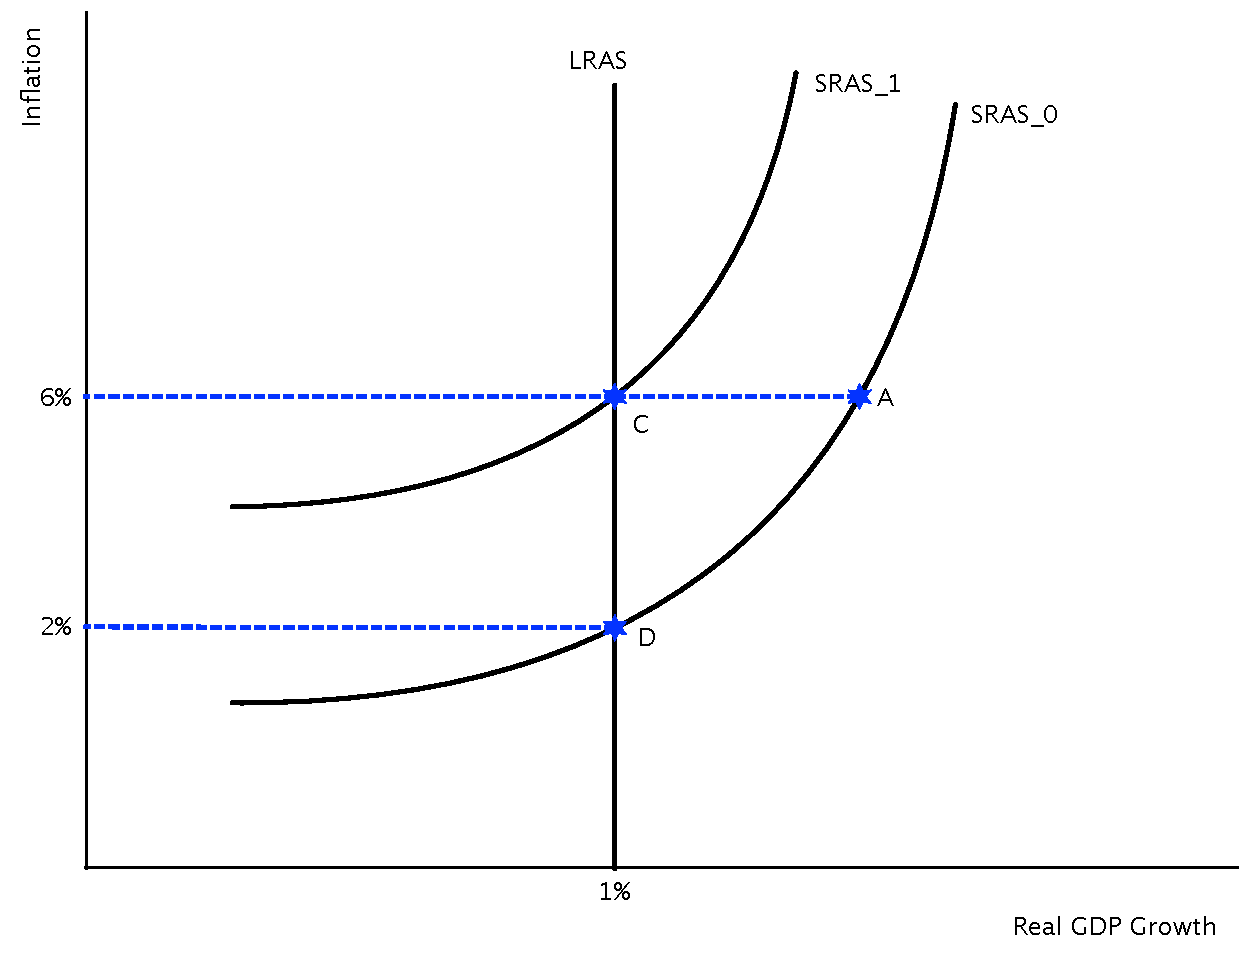
\includegraphics[scale=.40]{final_32.pdf}
	\caption{SRAS and LRAS}
	\label{fig5}
\end{figure}

Expected inflation at point $A$ is \blank, which is \blank actual inflation.

\begin{choices}
\choice 2\%; greater than
\choice 6\%; equal to
\choice 6\%; greater than
\CorrectChoice 2\%; less than
\end{choices}

\begin{solution}
Expected inflation is where SRAS and LRAS meet. $\pi^e = 2\%$ on $SRAS_0$, which is less than actual inflation of 6\% at point $A$.
\end{solution}

\question Suppose you lend your roommate \$100 for one year at 12\% nominal interest. You both expect the real interest rate on the loan to be 9\%. If at the end of the loan wealth was transferred from your roommate to you, then actual inflation over the course of the year could have been
	
\begin{choices}
		\CorrectChoice $0\%$.
		\choice $7\%$.
		\choice $9\%$.
		\choice $14\%$.
		\choice Either (a) or (b).
\end{choices}
	
\begin{solution}
$i = r^*  + \pi^e \Rightarrow \pi^e = i - r^* = 3\%$. If wealth is transferred from your roommate (borrower) to you (lender), then $\pi < \pi^e$ and so $\pi < 3\%$.
\end{solution}

\newpage

\question A country's output per worker is described by the function $y=2\sqrt{k}$. Capital depreciates at a rate of 2\% and the labor force remains the same each period. If the country sets a savings rate of 30\%, what will be the level of output per worker once the country reaches its steady state?

\begin{choices}
\choice 900
\choice 45
\CorrectChoice 60 
\choice 30
\end{choices}

\begin{solution}
Steady state where $i = d$. $i=sy = .30(2\sqrt{k})$ and $d=\delta k = .02k$ $\Rightarrow .6\sqrt{k} = .02k \Rightarrow k^* = (.6/.02)^2 = 900$. $y^* = 2\sqrt{900} = 60$.
\end{solution}

\question Refer to Table \ref{wtp}, which gives the willingness to pay for a Bun's milkshake for four individuals.
		
		\begin{table}[h!]
			\caption{WTP for Milkshakes}
			\label{wtp}
			\centering
			\begin{tabular}{  c|c    }    
				
				Buyer   & WTP \\
				\hline
				Buster & \$4.00 \\
				Michael & \$2.50 \\
				Lindsey & \$3.00 \\
				Gob & \$.50 \\
			\end{tabular}
			
		\end{table} 
		
		Suppose the price of milkshakes decreases from \$3.50 to \$2.00. The change in total consumer surplus that is due to buyers entering or exiting the market because of the price change is
		
		\begin{choices}
			\choice \$1.00.
			\choice \$3.00.
			\choice \$4.50.
			\CorrectChoice \$1.50.
		\end{choices}
		
\begin{solution}
Buys as long as $WTP > P$. At $P_0$ = \$3.50, only Buster is willing to buy a milkshake and realizes surplus of (4 - 3.50) = \$.50. At $P_1$ = \$2, Buster, Michael, and Lindsey are all willing to purchase and realize consumer surplus of (4 - 2) + (2.50 - 2) + (3 - 2) = \$3.50. Increase in surplus from Buster (old buyer): \$1.50. Increase in surplus due to new buyers: \$1.50.
\end{solution}

\question Which of the following is NOT an issue when implementing monetary policy?

\begin{choices}
\CorrectChoice Legislative lag
\choice Effectiveness lag
\choice Imperfect control over the money supply
\choice Implementation lag
\end{choices}

\begin{solution}
See class notes.
\end{solution}

\question There are two polluting firms, firm A and firm B, in the town of Wooten. The government decides to curtail pollution by distributing pollution permits to each firm which can be traded between the firms. If firm B buys all the pollution permits from firm A, which of the following is true?

\begin{choices}
\choice Firm A has a higher cost of reducing pollution than firm B.
\CorrectChoice Firm B has a higher cost of reducing pollution than firm A.
\choice The two firms have the same cost of reducing pollution.
\choice Comparing the firms' pollution costs is impossible without more information.
\end{choices}

\begin{solution}
See class notes. The firm with a higher cost of reducing pollution will buy permits from the firm with lower costs.
\end{solution}

\newpage

\question Which of the following accurately describes the relationship between the price, average total cost, and average variable cost for a firm in a perfectly competitive market given that the firm is currently producing output, but is making a loss?

\begin{choices}
\choice $ P > ATC > AVC$
\choice $ ATC > AVC > P$
\choice $ ATC = P > AVC$
\CorrectChoice $ ATC > P > AVC$
\end{choices}

\begin{solution}
Firm operates, but makes a loss if $AVC < P < ATC$ at the optimal quantity.
\end{solution}

\question Table \ref{MC23} shows the prices and quantities produced and consumed of the only two goods in Uzbeki-beki-beki-Stan-Stan, grapes and olives, for the years 2000 -- 2002.
	
	\begin{table}[h!]
		\caption{Grapes and Olives in UZN}
		\centering
		\begin{tabular}{c|c|c|c|c}
			Year & Grapes  & Price of Grapes & Olives  & Price of Olives \\
			\hline
			2000 & 20 & \$2.10 & 4 & \$4.10\\
			2001 & 19 & \$2.25 & 6 & \$4.15\\
			2002 & 22 & \$2.20 & 7 & \$4.15\\
		\end{tabular} 
		\label{MC23}
	\end{table}
	
	Using 2000 as the base year, real GDP in 2001 was \blank, while nominal GDP in 2002 was \blank.
	
	\begin{choices}
		\choice \$61.60; \$77.45
		\choice \$67.65; \$74.90
		\CorrectChoice \$64.50; \$77.45
		\choice \$61.60; \$74.90
		\choice \$64.50; \$74.90
	\end{choices}
	
\begin{solution}
Base yr: 2000. Real GDP is calculated using base year prices and current production, while nominal GDP is calculated using current year prices and production.\\
Real GDP 2001: $19\times(\$2.10) + 6\times(\$4.10) = \$64.50$.\\
Nominal GDP 2002: $22\times(\$2.20)+7\times(\$4.15) = \$77.45 $.
\end{solution}

\question Suppose your Aunt Stella gives you \$500 in cash. The minimum reserve requirement set by the Fed is 10\%, but banks choose to hold 12.5\% in reserves. What is the maximum potential \textit{increase} in the money supply if you choose to hold half your cash as a demand deposit?

\begin{choices}
\CorrectChoice \$1,750
\choice \$2,000
\choice \$2,250
\choice \$2,500	
\end{choices}

\begin{solution}
$MM = 1/rr = 1/.125 = 8$. Deposit \$250 $\Rightarrow$ max $\Delta MS = \$250\times 8 - \$250$ = \$1,750 (since you removed \$250 in currency).
\end{solution}

\question Assume an economy has a natural growth rate of 4\% and is currently at its long-run equilibrium. If spending growth along the current $AD$ curve is 4\%, then inflation must be \blank. Additionally, actual inflation is currently \blank expected inflation.

\begin{choices}
\choice 8\%; equal to
\choice 0\%; less than
\choice 8\%; greater than
\CorrectChoice 0\%; equal to
\choice None of the above.
\end{choices}

\question Suppose a wave of investor and consumer optimism has increased spending growth so that current output growth exceeds the long-run natural growth rate. If policymakers choose to engage in activist contractionary policy, they should

\begin{choices}
	\choice decrease taxes, which will shift aggregate demand to the left.
	\CorrectChoice decrease government spending, which will shift aggregate demand to the left.
	\choice decrease government spending, which will shift aggregate demand to the right.
	\choice decrease taxes, which will shift aggregate demand to the right.
\end{choices} 

\question Table \ref{MC43} shows the prices and quantities produced and consumed of the only two goods in Uzbeki-beki-beki-Stan-Stan, grapes and olives, for the years 2000 -- 2002.

\begin{table}[h!]
	\caption{Grapes and Olives in UZN}
	\centering
	\begin{tabular}{c|c|c|c|c}
		Year & Grapes  & Price of Grapes & Olives & Price of Olives \\
		\hline
		2000 & 20 & \$2.10 & 4 & \$4.10\\
		2001 & 19 & \$2.25 & 6 & \$4.15\\
		2002 & 22 & \$2.20 & 7 & \$4.15\\
	\end{tabular} 
	\label{MC43}
\end{table}

Assuming the typical basket of grapes and olives is determined by the quantity of each consumed in 2000, then the price level in 2001 used to compute the CPI is \blank.

\begin{choices}
	\choice \$67.65
	\choice \$64.50
	\choice \$58.40
	\CorrectChoice \$61.60
\end{choices}

\begin{solution}
	Price level calculated is using current year prices and fixed basket of goods.\\
	$P_{2001} = \$2.25\times(20) + \$4.15\times(4) = \$61.60$.
\end{solution}

\question In the presence of a savings tax credit, how many of the following are FALSE?
	
	\begin{enumerate}[(i)]
		\item The real interest rate will increase.
		\item The quantity of investment will decrease.
		\item The quantity of savings will increase.
	\end{enumerate}
	
	\begin{choices}
		\choice 0
		\choice 1
		\CorrectChoice 2
		\choice 3
	\end{choices}	
	
\begin{solution}
A savings tax credit will increase the supply for loanable funds. As a result, the real interest rate will decrease, while both savings and investment will increase.
\end{solution}

\newpage

\question Use the game matrix below to answer the question that follows.

	\renewcommand{\gamestretch}{1.5}
	\sgcolsep=25pt
	\begin{figure}[h!]\hspace*{\fill}%
		\begin{game}{3}{3}[Noah][Isabella] 
			&  Run & Walk & Crawl \\
			Run & 2, 1 & 4, 4 & 8, 2 \\
			Walk & 3, 0 & 1, 3 & 2, 2 \\
			Crawl & 3, 4 & 5, 5 & 4, 4 \\
		\end{game} 
		\hspace*{\fill}%
	\end{figure}
	
Which of the following statements are TRUE?

\begin{enumerate}[i.]
	\item Noah does not have a dominant strategy.
	\item Isabella does not have a dominant strategy.
	\item This game has no Nash equilibrium.
\end{enumerate}

\begin{choices}
\CorrectChoice Only i
\choice Only i and iii
\choice Only ii and iii
\choice i, ii, and iii
\choice None of the statements are true
\end{choices}

\begin{solution}
Noah does not have a dominant strategy. Isabella's dominant strategy is Walk. Noah's best response to this is Crawl, and so the NE is (Crawl, Walk).
\end{solution}

\question Sweet Dee's Ostrich farm can currently produce 500 ostrich eggs per day with 50 workers. If Dee hires 100 more workers, she can increase egg production by 1,000 eggs. The marginal product of labor per worker from these additional laborers is

\begin{choices}
\choice 1,000.
\CorrectChoice 10.
\choice 100.
\choice 15.
\end{choices}

\begin{solution}
$MP_L = \Delta Q/\Delta L = 1,000/100 = 10$.
\end{solution}

\question When an increase in government spending increases the income of some people, and those people spend some of that increase in income on additional consumer goods, we have seen a demonstration of 

\begin{choices}
\choice the investment accelerator. 
\CorrectChoice the multiplier effect.
\choice the crowding out effect.
\choice supply-side economics.
\end{choices}

\begin{solution}
See class notes.
\end{solution}

\question If GDP in Denmark was \$20,000 in 1988 and \$80,000 in 2016, then the country's \textit{annual} growth rate was approximately \blank during this period.

\begin{choices}
\choice 2.5\%
\choice 300\%
\choice 25\%
\CorrectChoice 5\%
\end{choices}

\begin{solution}
Quadruple time: 2(70/g) = 140/g = (2016-1988) = 28 $\Rightarrow$ g = 140/28 = 5\%.
\end{solution}

\newpage

\question Consider Figure \ref{fig6}.


\begin{figure}[h!]
	\centering
	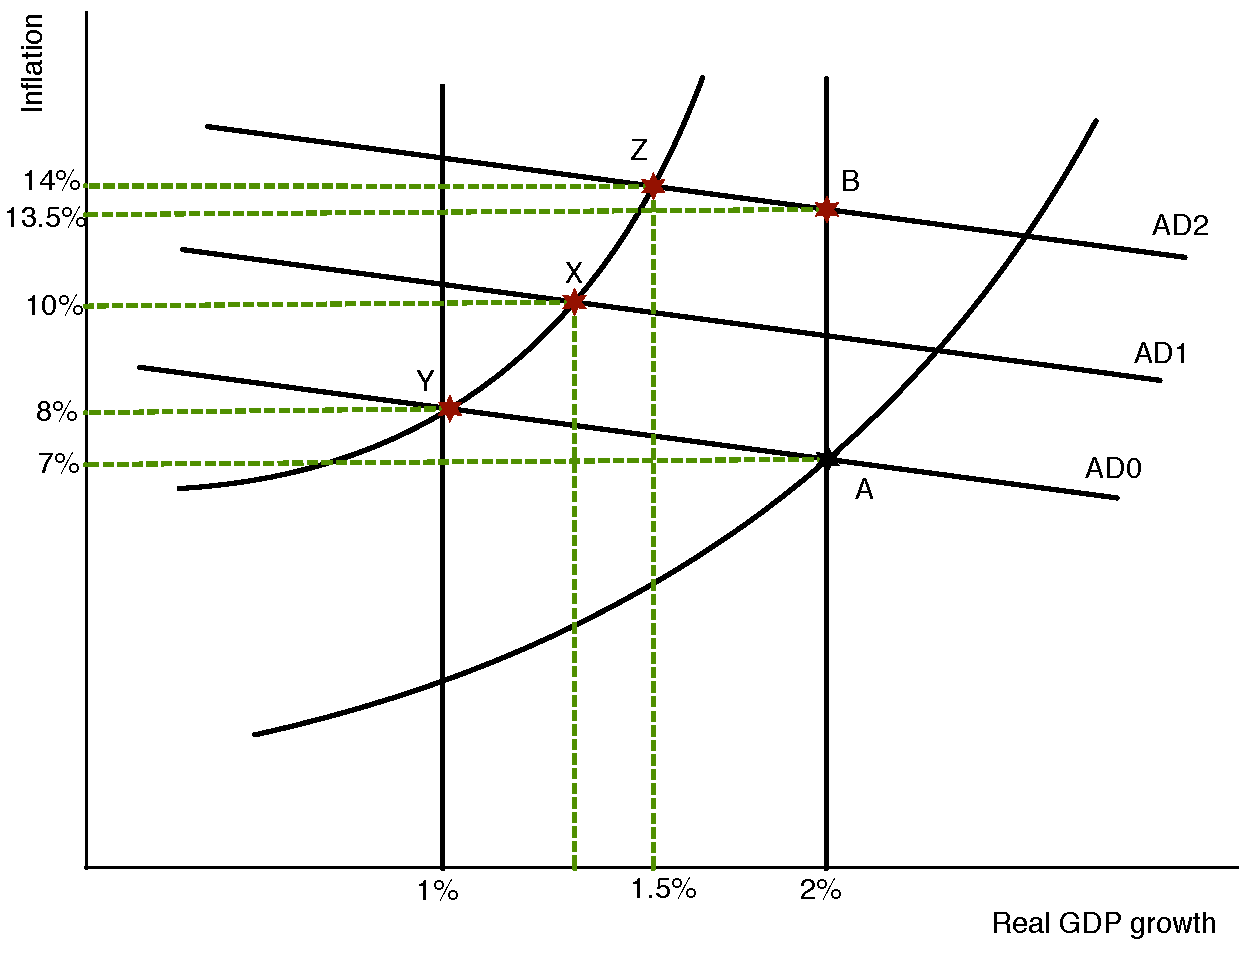
\includegraphics[scale=.45]{ec2_plot1.pdf}
	\caption{Real Shock}
	\label{fig6}
\end{figure}

If after a real shock the economy is operating at point $Y$, then, in the absence of crowding out, fiscal policy that shifted $AD0$ to $AD2$ would lead to inflation of \blank in the short run.

\begin{choices}
	\CorrectChoice 14\%
	\choice 10\%
	\choice 13.5\%
	\choice 8\%
\end{choices}

\begin{solution}
Real shock moved LRAS curve from $g=2\%$ to $g=1\%$. Long-run Eq at $AD0$ is $Y$. If AD shifts to $AD2$, economy would be where $AD2$ and the new SRAS curve intersect at point $Z$.
\end{solution}

\question Consider Figure \ref{fig7}.


\begin{figure}[h!]
	\centering
	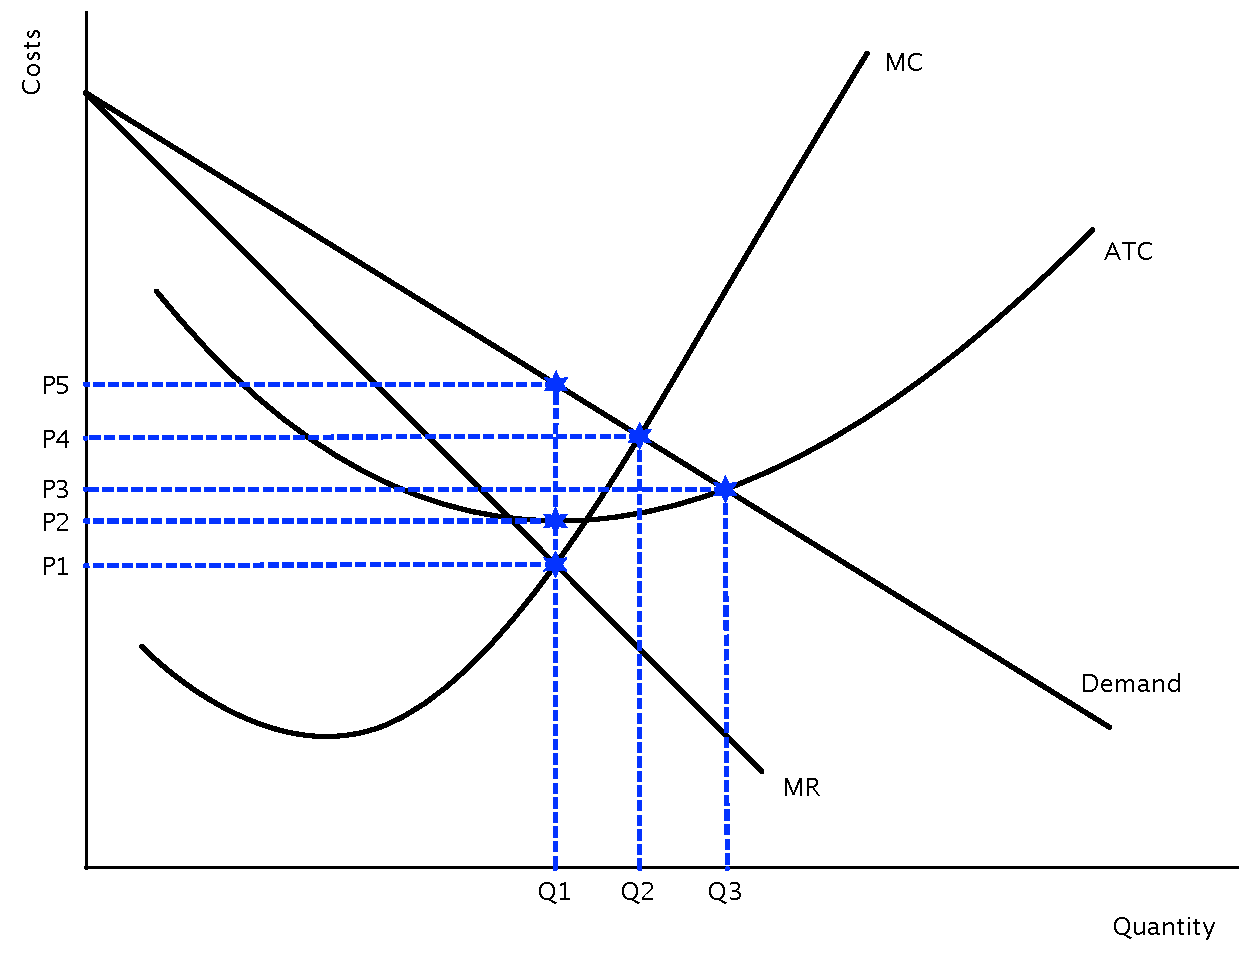
\includegraphics[scale=.45]{final_50.pdf}
	\caption{Monopolist Environment}
	\label{fig7}
\end{figure}

Which of the following represents the monopolist's profit at their optimal production level?

\begin{choices}
\choice $(P5 - P1)\times Q1$
\choice $(P4 - P2)\times Q2$
\CorrectChoice $(P5 - P2)\times Q1$
\choice $(P3 - P2)\times Q3$
\end{choices}

\begin{solution}
Produce at $Q1$ since that's where $MR=MC$. Charge $P5$ on demand curve. ATC at $Q1$ is $P2$.
\end{solution}

\end{questions}	

\section*{Short Answer}

For this section, make sure to write legibly and box final answers. \textbf{Show your work!} This can be done within the section or \textit{clearly} labeled on the scratch paper provided.

\begin{questions}

\question Suppose that an economy has a natural growth rate of 1\%. Moreover, the central bank in the country has perfect control over the money supply and increases it by 3\% every year. The economy's growth rate of real GDP is currently $-2\%$ and inflation is 1\%. Assume that any changes leading to the current rate of output growth and inflation are permanent. 
	
\begin{parts}
		
		\part[2] Is the economy currently at its long-run equilibrium? Explain why or why not.
		
		\begin{solution}[.5in]
		No. The current rate of output growth is less than the long-run natural growth rate of the economy.
		\end{solution}
		
		\part[2] What is current spending growth in the economy?
		
		\begin{solution}[.5in]
			Spending growth = $\vec{M} + \vec{v} = \pi + \vec{Y}_R = 1\% + (-2\%) = -1\%$.
		\end{solution}
		
		\part[2] What is the current rate of velocity growth?
		
		\begin{solution}[.5in]
			$\vec{M} + \vec{v} = -1\% \Rightarrow \vec{v} = -1\% - (3\%) = -4\%$.
		\end{solution}
		
		\part[2] What is the relationship between expected inflation and actual inflation at the point the economy is currently operating (i.e., which one is greater)?
		
		\begin{solution}[.5in]
			Expected inflation is greater than actual inflation.
		\end{solution}
		
		\part[4] Discuss how your answer to (d) relates to the economy's current rate of output growth.
		
			\begin{solution}[1in]
				Since $\pi^e > \pi$, firm profits are falling (e.g., wages rising faster than prices) and thus short-run growth is below the natural growth rate of output.
			\end{solution}
		
		\part[2] In the absence of monetary or fiscal policy interventions, what will the growth rate of output and inflation rate be in the long run?
		
			\begin{solution}[1in]
				In the long run, $\vec{Y}_R = g = 1\%$. Since spending growth is $-1\%$, inflation in the long run must be $-2\%$.
			\end{solution}
			
		\part[2] Suppose the central bank wishes to bring the economy back to its original long run equilibrium where long-run inflation was 2\%. State two policies they could enact in order to achieve this goal.
		
		\begin{solution}[1in]
			In order to increase AD, the central bank must increase $\vec{M}$. To do so, they can (i) engage in open market purchases, (ii) decrease the discount rate, (iii) decrease interest on reserves, (iv) decrease the minimum reserve requirement, or (v) decrease the Federal funds rate.
		\end{solution}
		
		\part[2] Regardless of the policy pursued, what will be the new rate of money growth the central bank must enact in order to achieve their goal?
		
		\begin{solution}[.5in]
			Spending growth at the new long-run equilibrium = 2\% + 1\% = 3\%. $\vec{M} + \vec{v} = 3\%$, so if $\vec{v} = -4\%$ then $\vec{M} = 7\%$.
		\end{solution} 
		
		\part[5] Draw a well-labeled AS-AD graph that shows the economy operating at their initial real GDP growth rate of $-2\%$ and inflation of 1\%, labeling this point $A$. Make sure to include the AD, SRAS, and LRAS curves. If different, label the long-run equilibrium point in the absence of government intervention point $B$. Finally, label the long-run equilibrium point if the central bank intervenes as you've described in (g) and (h) point $C$. \textit{Make sure to clearly show what the inflation rate and rate of output growth is at each point as well as any shifts in the AD, SRAS, or LRAS curves.}
		
			\begin{solution}[2.5in]
				
			\end{solution}
			
			\dd{\begin{figure}[h!]
					\centering
					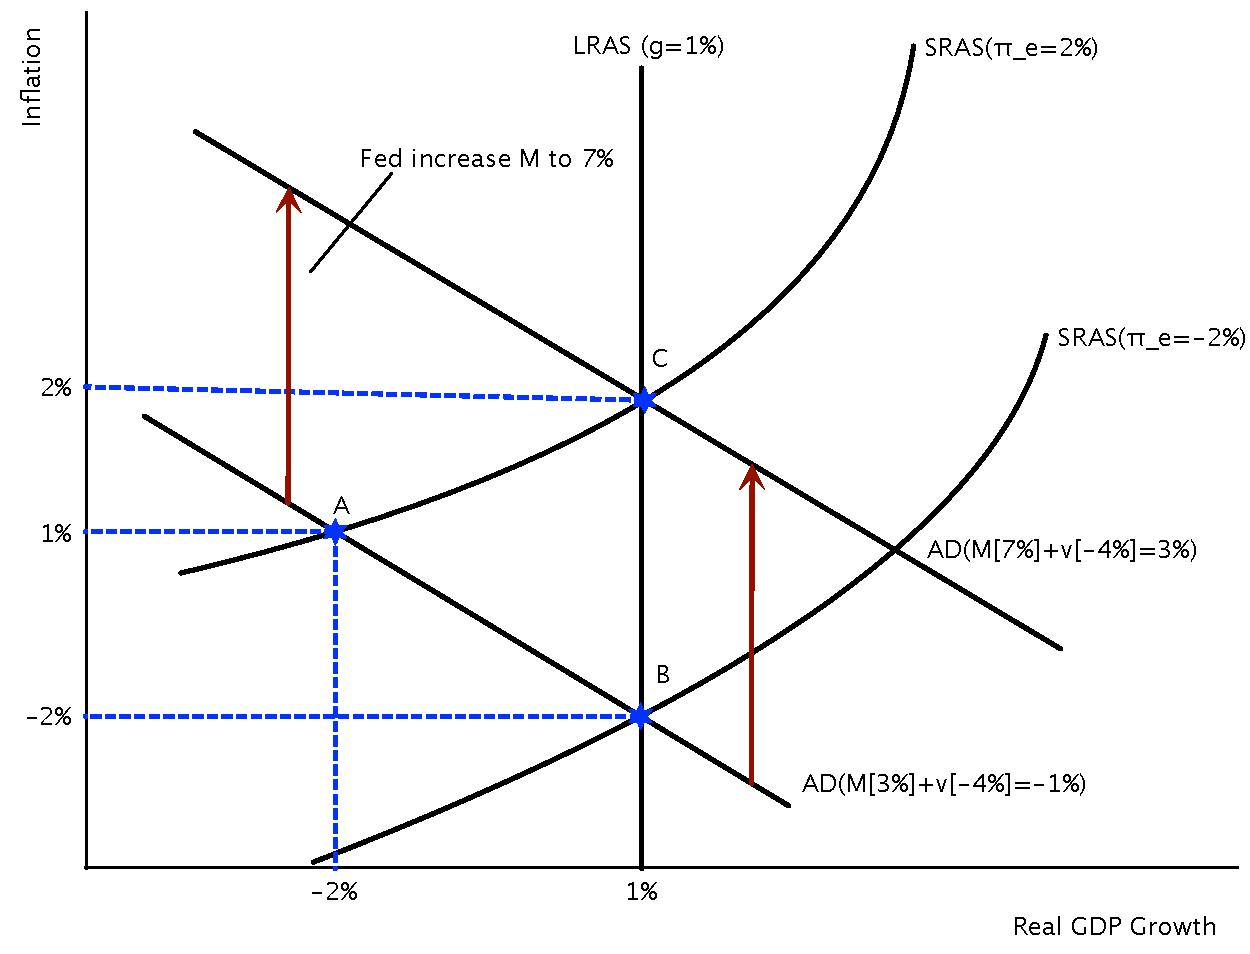
\includegraphics[scale=.45]{final_sa.pdf}
					\caption{AS-AD Plot}
					\label{fig8}
				\end{figure}}
		
		\part[2] What is the expected inflation rate at points $A$, $B$, and $C$ in your plot from (i)?
		
			\begin{solution}[.5in]
				Expected inflation at $A$ = expected inflation at $C$ = 2\%. \\
				Expected inflation at $B$ = $-2\%$.
			\end{solution}

\end{parts}
		
\end{questions}

\hrulefill
\begin{center} 
	\textbf{END OF EXAM}
\end{center}

\newpage

\centering

\section*{SCRATCH SHEET}


\end{document}